\documentclass[12pt,a4paper]{article}
\usepackage[utf8]{inputenc}
\usepackage{graphicx}
\title{Math@Cpt}
\author{maryklayne }
\date{November 2014}
\usepackage{natbib}
\usepackage{graphicx}

\sloppy

\title{Mitigando a Evasão de Alunos de Computação Devido às Disciplinas Matemáticas}

\author{Anderson Silva, 
Carlos Henrique, 
Elthon Allex,\\
Fillipe Dos Santos, 
Maryklayne Araujo, 
Wanne Cleia}



\begin{document} 

\maketitle

\section{Introdução}
Desde o início de suas aulas em 18 de setembro de 2006, o curso de Ciência da Computação vem funcionando na sede do Campus Arapiraca, da Universidade Federal de Alagoas. Os alunos que ingressam neste curso são, em sua maioria, provenientes de escolas públicas do interior de Alagoas. Desde então, os professores deste curso e do curso de Licenciatura em Matemática perceberam uma enorme deficiência dos alunos ingressantes em conteúdos matemáticos. Numa pesquisa preliminar, foi constatado que cerca de 78\% dos alunos entrevistados alegaram ter tido um  aproveitamento ruim ou regular nas disciplinas matemáticas de Computação. Isto acaba fazendo com que os alunos não consigam dar prosseguimento aos seus estudos no curso devido aos problemas enfrentados em aprender os conteúdos abordados em muitas das disciplinas, tais como: Cálculo 1, Matemática Discreta, Geometria Analítica, Álgebra Linear, Computação Gráfica, dentre outras. Devido a isso, o curso vem apresentando um baixo índice de egressos, um alto índice de retenção e um índice relativamente alto de evasão. Este projeto, intitulado Math@Cpt, pretende melhorar este cenário definindo e executando ações de intervenção junto aos alunos do curso de Computação e professores dos cursos de Computação e Matemática.

\section{Trabalhos na área de ensino de Matemática}

\subsection{Dificuldades Em Aprender e Ensinar Matemática}
Esta trabalho apresenta as principais dificuldades observadas no processo de ensino-aprendizagem da Matemática, visando encontrar soluções para os devidos problemas.
Dentre as dificuldades citadas no trabalho, o fato do aluno não estudar o conteúdo matemático dentro da sua realidade, acaba levando para o desinteresse, pois o ensino em qualquer área, deve acontecer de forma que o mesmo sinta a necessidade de aprender algo, e este aprendizado deve ser voltado para seu dia a dia, fazendo com que perceba a importância da disciplina para a sua vida. 
Outra queixa constantemente é a complexidade no ensino matemático devido a utilização de vários exercícios repetitivos e também de utilização de fórmulas tornando a Matemática bastante mecânica e pouco explicativa. 
Das soluções propostas, se o professor ministrar as aulas de forma que o aluno precise pensar e assimilar diferentes meios de resoluções de problemas de um determinado conteúdo, com esse procedimento o aprendiz estará desenvolvendo seu raciocínio lógico . Ao apresentar os conteúdos,o professor deve procurar melhores formas de transmitir o conhecimento, pois dentro de uma sala de aula existem alunos com várias habilidades como também há aqueles com diversas dificuldades, é importante que o docente busque manter um bom nível de aprendizado para todos.
O artigo conclui que, é conveniente que o professor trabalhe sempre buscando um ponto de vista focado na necessidade e na realidade do estudante, tornando o ensino matemático cada vez mais atual. O aluno ligado às modernidades tecnológicas terá maior facilidade em encontrar utilidade no que está aprendendo. SEM REFERENCIA

\subsection{Matemática: Uma Disciplina Condenada ao Insucesso?}
O trabalho apresentado dispõe-se em retorquir sobre quais as causas que torna a disciplina de Matemática sem sucesso e um meio desse problema ser contestado. Apresenta de forma geral, a opinião entre professores, pais e discentes sobre o que pensam à respeito do insucesso que predomina nesta disciplina.
Verificou-se que para os professores os fatores do insucesso dos alunos são constantemente a sua má preparação em anos anteriores, ao mesmo tempo apontando o fato de muitas famílias possuírem um nível sócio-econômico e cultural muito baixo, os professores mencionam que os alunos não se esforçam, não prestam atenção nas aulas nem estudam em casa, contestando também os currículos de serem excessivamente longos e que a obrigação de seu cumprimento faz com que deixem para trás os aprendizes  mais lentos. 
Para os alunos o insucesso da Matemática é o fato da disciplina ser assustadoramente difícil de entender, os professores não explicam bem e nem a torna cativante, contudo não conseguem perceber para que serve e nem conseguem saber o motivo pelo qual são obrigados a estudá-la.
Para os pais e para a opinião pública em geral, a culpa está nos professores que não ensinam adequadamente, porém todos reconhecem que é uma disciplina complicada e que a sua aprendizagem tem causado enormes dificuldades em todas as gerações. 
Para o autor a razão fundamental do insucesso é que a disciplina é configurada propriamente para levar ao insucesso, resultando da função que lhe é concebida no sistema educacional, as aulas de 50 minutos não auxiliam na realização de atividades que exigem maior concentração e tempo superior, nem trabalho em grupo , nem a utilização de novas tecnologias. Fazendo com que os educandos enxerguem a Matemática como um mero amontoado de regras sem qualquer relação entre si, querem até saber como faz os exercícios, porém, acham que nem vale à pena tentar entender a lógica que liga os diferentes assuntos. 
E ainda nesse contexto, João Pedro da Ponte acredita ser possível tornar o ensino desta disciplina de modo à se reintegrar como uma experiência escolar de sucesso, fomentando uma visão da Matemática como uma ciência em permanente crescimento, sendo necessário: 
- Criação de uma imagem diferente da Matemática,
- Divulgação de uma visão mais ampla 
- Formação dos professores para uma nova visão em Matemática 
- Reformulação de currículos 
- Diversidade das formas e instrumentos de avaliação 
Concluindo-se que o insucesso causado,está também no papel social que lhe é atribuído, é maneira com ela se relacionam e como é vista pelos diversos autores e para combater essa frustração a principal medida é retirando-lhe esta função devastadora e mostrando como essa ciência pode constituir uma atividade intelectual gratificante e enriquecedora. SEM REFERENCIA

\subsection{O uso da Geometria Interativa como Facilitador no Ensino e Aprendizagem de Matemática: 
estudo com duas turmas de sexta série do ensino fundamental}

Este artigo apresenta uma tentativa de ensino e aprendizagem de geometria, com ajuda das tecnologias da informação e comunicação, sendo os envolvidos alunos da sexta série do Ensino Fundamental. 
Foi feito um experimento cuja motivação foi resolver, de modo intuitivo um problema de otimização de área, envolvendo conceitos e limites de convergência. Paro o projeto de ensino foi escolhido o iGeom(geomeria interativa na internet), sistema gratuito de geometria e interativo, e sistema SAW(sistema de aprendizagem pela web).
Do resultado, o uso dessas duas ferramentas possibilitou a motivação dos alunos ao receberem rapidamente retorno sobre suas atividades, com o recurso de feedback e verificou-se que o sucesso do experimento se deu através da atividade que por sua vez era interativa, outro ponto foi que os alunos conseguiram avançar além do conteúdo curricular, em função da agilidade proporcionada pelas TICs.\citep{tanbellini2010uso}

\subsection{REPROVAÇÃO E EVASÃO NO ENSINO MÉDIO NA CIDADE DE  RIBEIRÓPOLIS – SERGIPE}
Desde os anos iniciais básicos escolar, houve-se frequentemente sobre as dificuldades enfrentadas pelos alunos na disciplina de Matemática, tais dificuldades que continuam a crescer quando o aluno chega ao ensino médio e superior. Preocupados com o alto nível de evasão e reprovação escolar, a equipe se propôs a realização de um pesquisa com os alunos de 1º,2º e 3º ano do ensino médio na cidade de Ribeirópolis no estado de Sergipe, com o objetivo de unir respostar e entender por parte dos mesmos quais as maiores dificuldades enfrentadas com a disciplina em questão e qual seria uma melhor solução para combater o problema.
Do resultado da pesquisa, verificou-se que a falta de incentivo ao pensamento lógico é um dos maiores problemas e metodologias de ensino inadequado. Houve convergência entre respostas, 87\% dos alunos entrevistados confirmaram nunca terem sido reprovado na disciplina em questão, e 67\% dos alunos disseram que o maior índice de reprovação era na disciplina em questão. 
Surgiram algumas propostas para combater o problema da evasão e reprovação pelos alunos questionados, uma das soluções seria tornar as aulas mais interativas, para o aluno compreender melhor a Matemática, e que a mudança de avaliação poderia dar fim o grande número de reprovação, a maior parte dos alunos entrevistados responderam que o aprendizado e incentivo que recebem não seriam suficiente para que eles se dedicassem. 
A equipe constatou que mesmo com a grande dificuldade enfrentadas pelos alunos,o índice de reprovação era baixo e portanto o conhecimento do alunos também era baixo.\citep{santosreprovaccao}

\subsection{Universidade da MadeiraDepartamento de Ciências da EducaçãoMódulo  II- Organização e Administração EscolarCurso: Mestrado em Ensino da Matemática Prof. Antônio Bento}
Este trabalho é uma apresentação de mestrado, cuja a equipe pretende verificar quais as causas do insucesso no ensino de matemática, e o porquê da dificuldade enfrentada pelo aluno. 
 Através de um levantamento bibliográfico, verificou-se algumas causas que levavam ao insucesso, como condições de ensino e condições de aprendizagem, não se pode forçar o aluno a estar em uma atitude passiva e unicamente de receptor além de ser perda de tempo é uma das causas do insucesso, ou seja não se aprende se não estiver envolvido, só aprendemos o que vivemos o resto esquecemos, outra causa do insucesso é a introdução precoce das máquinas de calcular aos estudos do aluno.
Com o desejo de conhecer a opinião daqueles que sentem na pele o insucesso e as dificuldades que se mostram na disciplina de Matemática, a equipe realizou uma pesquisa com quarenta alunos da escola secundária Jaime Moniz, no qual a condição especial de serem alunos do 10º à 12º ano que se encontram a repetir a disciplina e no resultado da pesquisa , 18 alunos responderam que a motivação pela disciplina era média, 54\% responderam que o método habitual de ensino era resoluções de exercícios, 75\% afirmaram não ter apoio na escola, 60\% disseram não ter ajuda, e dos alunos que responderam ter ajuda, 7 responderam ser dos pais, ficando o professor em 3º lugar com três alunos, 65\% dos alunos afirmaram que a falta de motivação era o principal fator da causa do insucesso, 63\%  responderam ser a falta de base, 50\% falta de estudos e resultados negativos. 
Na opinião de 33 professores questionados, 26\% responderam que a culpa era do método de ensino, 24\% a falta de motivação para o aluno, 21\% tempo insuficiente para resoluções de problemas. 
Com a pesquisa concluiu-se que as causas do insucesso na disciplina ,são multifatoriais: aluno, professor, sistema escolar, família e sociedade. No questionário realizado à 40 alunos do ensino secundário, sendo todos repetentes da disciplina a maioria apresenta pouca ou nenhuma motivação com a disciplina, a maioria não tem ajuda para estudar , e quando essa ajuda existe é facultado por um familiar ou explicador, foi identificado como causa do insucesso a desmotivação dos alunos, falta de bases, falta de estudo e o acumular dos insucessos. Entretanto, os professores também são responsáveis pelo método de ensino utilizado, pela incapacidade em motivar os alunos e pelo pouco de tempo utilizado para resolução de problemas. REFERENCIA NAO ENCONTRADA

\subsection{Discussões sobre modelagem matemática e o ensino-aprendizagem}
Este trabalho apresenta a modelagem como uma solução para que os alunos compreendam a importância e o uso da matemática no seu cotidiano, já que muitos não têm o interesse de aprender, devido à falta de incentivo ou mesmo da insuficiência de ferramentas que os ajudem no aprendizado. Acredita-se que trabalhando os conceitos matemáticos à partir da ralidade em que vivem, a Matemática passa à ser mais interessante e sedutora aos olhos dos mesmos, pois são capazes de contribuir na própria construção do saber ao qual estão tendo contato. 
Os benefícios que a modelagem proporciona, citados pelos autores são: Motivação dos alunos e dos próprios professores, facilitação de aprendizagem, pois o assunto deixa de ser abstrato e passa a ser concreto, preparação para futuras profissões, desenvolvimento do raciocínio lógico, dedutivo e geral. 
Contudo, os autores se preocupam com alguns desafios à serem vencidos para que os objetivos possam ser alcançados, são eles, à falta de apoio das instituições de ensino, desmotivação por parte dos professores que exercem uma carga excessiva de horas de trabalho, falta de interesse por partes dos alunos, indisciplina, falta de tempo para elaboração de projetos alternativos de ensino, resistência de outros professores acostumados com o ensino tradicional, Programa do currículo previamente estabelecido, não dando a oportunidade do professor variar sua metodologia de ensino, sendo necessário cumprir o programa que é inflexível.\citep{silveira2005discussoes}

\subsection{O Ensino da Matemática com Significação nos Anos Iniciais da Educação Básica}
Este trabalhado discute sobre como deve acontecer o processo de ensino-aprendizagem da matemática nos alunos de Educação Básica, para que construam seu pensamento lógico-matemático de forma organizada, acreditando-se que, só será possível uma aprendizagem de qualidade, se os alunos entrarem em contado com atividades que possam manipulá-las e ao mesmo tempo fazer relações de situações que os rodeiam, fazendo com que esse processo de aprendizagem lhes sejam agradável. 
Mas ainda verifica-se uma objeção na construção do conhecimento, pois a técnica utilizada por muitos professores ainda é a tradicional, não utilizam nenhum meio de ensino voltado para a prática. Entretanto, há aqueles docentes preocupados com as críticas devidos esses resultados negativos, e se comprometem a buscarem soluções para tal dificuldade que o aluno de ensino básico enfrenta, procurando ensinar matemática voltada à sua realidade.\citep{santos2008ensino} 

\subsection{Refletindo Sobre as Dificuldades de Aprendizagem na Matemática: Algumas Considerações}
Das mudanças ocorridas no ensino da Matemática desde as décadas de 40 à 90, e nesta última, foi verificado que não era das tarefas de cálculo que os alunos tinham os piores resultados, mas nas tarefas de ordem complexa, que exigiam algum raciocínio, flexibilidade e espírito crítico.
Neste trabalho, almejou-se refletir sobre alguns dos aspectos que habitualmente dificultam a aprendizagem da matemática, são eles, o preconceito de que matemática é difícil, formação inadequada de professores, uso da metodologia tradicional, pouco incentivo, entre outros. Concluindo-se que a dificuldade aumenta ainda mais, quando a matemática é ensinada sem explicitar a origem e finalidades dos conceitos, surgindo a necessidade de um ensino associado à história da matemática.\citep{silva2005refletindo}

\subsection{Softwares Livres Potenciais para o Ensino de Matemática}
Com a preocupação existente por partes de alguns professores e pesquisadores em fazer o uso inteligente do computador em sala de aula, com o objetivo de fazer desse recurso uma possibilidade de melhorar o ensino aprendizagem, este artigo tem como foco principal à identificação, seleção e classificação de softwares livres disponíveis na Internet, promovendo o acesso e capacitando os usuários para o uso desses softwares. 
Dentre os softwares selecionados estão :
- Explorando conceitos da trigonometria através de software livres
- Funções trigonométricas inversas em ambiente informatizado
- Análise algébrica e geométrica das soluções de sistemas lineares utilizando o software Winplot.
- Explorando conceitos de trigonometria
- Estudo das funções trigonométricas
- Cálculo do volume de um sólido de revolução\citep{dosciatisoftwares}

\section{Relação entre matemática, alunos, dificuldades enfrentadas pelos professores}
Sem dúvida a matemática é uma das disciplinas que mais aborrece estudantes, por julgarem ser difícil, obscura e muitas vezes presumirem a matemática como supérflua. Dessa forma, restando-lhes apenas o ódio e o desânimo em compreender a verdadeira importância da matemática. 
Por se fazer presente em diversos aspectos da vida cotidiana acaba por ganhar grande prestígio na sociedade, e o que muitos alunos não querem enxergar é que utilizam, por mais simples que sejam, conhecimentos matemáticos em suas atividades do dia a dia. Se olharmos em nossa volta, encontramos matemática quase em tudo que vemos, desde um simples objeto com sua forma, tamanho, largura entre outros aspectos ou na construção de uma casa, por exemplo. 
A complexidade da matemática é utilizada de acordo com as nossas necessidades. Deste modo, não podemos nos restringir em apenas determinados conteúdos por achar outros difíceis, e sim encontrar meios para que a matemática possa se tornar familiar em nossas vidas. Com isso, excluindo a ideia de que matemática é difícil e inútil.
O gosto da matemática pelo estudante, nasce à partir dos primeiros anos inicias da sua vida escolar. Onde vai depender de como as informações foram transmitidas para os próprios e do processo de adaptação com a disciplina.Mas o que se pode notar é que entre uma quantidade excessiva de alunos, há uma grande dificuldade entre assimilar o uso da matemática para a vida pessoal e profissional. Gerando assim, um alto índice de reprovações e desinteresse na disciplina.
No entanto, percebe-se que os métodos utilizados para aprendizagem do aluno não estão surtindo efeitos favoráveis. Já que ao progredirem para anos mais avançados, as dificuldades e o desinteresse em aprender só aumentam, levando a disciplina ao insucesso.
Outro fator identificado, no que diz respeito ao fracasso na disciplina, foi a aprovação de alunos, mesmo não estando preparados para a introdução de novos conteúdos matemáticos. Afirma o artigo que aborda sobre a reprovação e evasão no ensino médio na cidade de Ribeirópolis-Sergipe.
"A desistência de solucionar um problema matemático é causada por um acúmulo de desinformação mas esse problema pode ser revertido, se acreditássemos e supervalorizássemos o poder da matemática formal. O mesmo em questão ocorre, por que muitos alunos são aprovados pelas disciplinas sem a menor aptidão na mesma, com grandes dificuldades” (Santos gildean e col, 2009 ).
O insucesso na disciplina, por sua vez, é conduzido através de uma série de fatores. E um desses fatores pode estar relacionado com os primeiros anos iniciais escolar do aluno, pois é neste período que o aluno estará desenvolvendo seu raciocínio lógico. As ações que as crianças e os jovens adoram, como, movimentar-se, conversar, perguntar, rabiscar, brincar, colorir, cantar, jogar e principalmente agir, tornam-se veículos surpreendentes para o aluno aprender. Uma vez que proporciona alegria e satisfação na criança.(Santos, sueli,2007) 
Portanto é preciso que o professor utilize métodos de ensino onde o aluno possa participar dinamicamente da aula com atividades que lhe conduza ao interesse em aprender, fazendo analogias do que lhe é apresentado dentro da sala de aula com o mundo ao seu redor.
“O conhecimento matemático tem que ser construído pelo aluno por meio de atividades que                                 lhe despertem o interesse para aprender. Fazendo relações do que ele vê dentro da escola com o que ele já conhece fora da escola. Compartilhado  por ele no seu convívio sócio cultural”(santos sueli, 2007).
Entretanto, percebeu-se que a grande maioria dos professores utilizam métodos tradicionais de ensino, deixando o aluno apenas na posição de ouvinte,  o que acaba tornando a aula muito mecânica e por sua vez desagradável.    
                 “Um grande número de professores tem como único objetivo ensinar Matemática sem se preocuparem em repassar para o aluno um conhecimento significativo, mesmo por que sentem muita dificuldade em relacionar o conteúdo apresentado teoricamente com a prática educacional, visto que os programas de formação em sua grande maioria não incorporam situações práticas durante todo o processo de  formação deixando uma vasta lacuna na formação do educador.” (Santos jamison e  col, s.d)
A Matemática dissociada da realidade é uma ciência isolada, sem sentido. Dessa forma ela carece de estímulos para o seu aprendizado. E para que gere estímulos é necessário que o professor seja altamente criativo e cooperador. Precisando assim, reunir habilidades para motivar o aluno, ensinando-o a pensar e a se tornar um autônomo. (Silva, 2005).
Mas em meio à tantas resistências, há professores e pesquisadores que se preocupam com os resultados devastadores em relação a Matemática, e com essa preocupação tendem à buscar novos métodos que possam auxiliar na aprendizagem do aluno.
Existem trabalhos que concentram-se fortemente em encontrar as causas principais que afetam o desempenho em matemática. Ao mesmo tempo em que pesquisa formas de adaptação do aluno com a disciplina em questão, com o objetivo de facilitar a aprendizagem, proporcionar gosto e mostrar a verdadeira importância da matemática para a vida. 
Dentre os fatores que afetam a aprendizagem, pode-se destacar o conceito pré-formado que a matemática é difícil, a capacitação inadequada de professores, a metodologia tradicional com ênfase no cálculo e a falta de contextualização. Uma solução seria uma disciplina lecionada de forma associada às necessidades da comunidade estudantil, a fim de capacitar os indivíduos para uma plena participação na vida social.(Silva,2005) 
A modelagem no ensino de matemática, por exemplo, poderia ser utilizada para que o aluno compreenda a importância e o uso da matemática no seu cotidiano. Acredita-se que, trabalhando os conceitos matemáticos dentro da realidade em que vivem os alunos, a matemática passa à ser mais interessante. A motivação do aluno e do professor, a facilitação de aprendizagem, preparação para futuras profissões, desenvolvimento do raciocínio lógico, dedutivo e geral podem ser vistos como benefícios proporcionados pela modelagem.(Carlos e Domin,2004)
Para melhorar o ensino e a aprendizagem do aluno, o uso inteligente do computador poderia ser utilizado em sala de aula. Através da identificação, seleção e classificação de softwares livres disponíveis na internet.
“Os professores de matemática precisam saber usar na sua prática  diferentes  recursos, como por exemplo, recursos computacionais, conhecendo as suas  possibilidades/potencialidades e aprendendo a usá-los com confiança. Nesse sentido, o computador é um importante aliado nesse processo, desde que possibilite mudanças no sistema atual de ensino, sendo usado pelo aluno para construir o conhecimento, ou seja, um recurso com o qual o aluno possa pensar, criar e manipular a informação.”(Dosciati e col, 2010).
Conclui-se que, é preciso que o aluno se relacione com os conteúdos matemáticos vistos em sala de aula de forma mais interativa. Trabalhando os conceitos à partir da realidade em que vive, a matemática passa à ser mais atraente. Dessa forma, proporcionando a curiosidade em descobrir, favorecendo a aprendizagem. É necessário a utilização de métodos que, por sua vez faça o aluno enxergar matemática de um modo mais concreto, dessa forma o aluno estará desenvolvendo seu conhecimento   de um jeito mais dinâmico, e poderá deixar de lado a ideia de que a matemática é inútil e difícil.

\section{Impacto da matemática na Ciência da Computação - UFAL}

Foi desenvolvido o formulário “Ensino de Matemática no curso de Ciência da Computação da Universidade Federal de Alagoas - Campus Arapiraca”, pelo aluno da UFAL Fernando Junior. Esse formulário tem o objetivo de identificar qual o ponto de vista dos alunos de Ciência da Computação com relação à matemática e possuiu uma amostra de 100 alunos. 

\begin{figure}[!h]
\centering
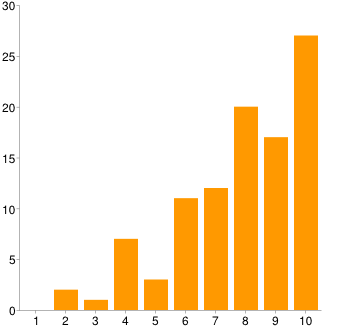
\includegraphics[scale=0.4]{imagens/fig1.png} 
\caption{Concepção de importância da matemática }
\end{figure}

A maioria das respostas foram obtidas dos alunos do segundo período (29\%), representado na Figura 2. Para 27\% dos alunos o nível de importância da matemática no seu curso foi máxima, onde nenhum aluno acha que ela é dispensável, observe a Figura 1, dentre eles apenas 13\% achou que o grau de importância está entre 1 e 5. 

\begin{figure}[!h]
\centering
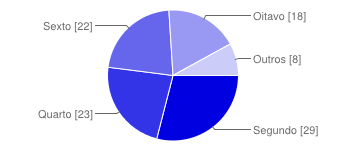
\includegraphics[scale=0.6]{imagens/fig2.png} 
\caption{Período atual do aluno }
\end{figure}

Apesar de 27\% dos alunos responderem que a importância da matemática é máxima, apenas 13\% tem esse mesmo grau de interesse de estudá-la, veja Figura 3. Considerando um grau de interesse bom entre 8-10, ficamos com um total de 45\% de alunos realmente interessados em se dedicar. 

\begin{figure}[!h]
\centering
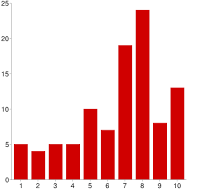
\includegraphics[scale=0.65]{imagens/fig3.png} 
\caption{Grau de interesse de estudar matemática}
\end{figure}

Segundo 51\% dos alunos, as disciplinas estudadas no curso suprem apenas algumas necessidades deles, em relação aos conteúdos matemáticos necessários para as disciplinas específicas de computação, representado na Figura 4. 

\begin{figure}[!h]
\centering
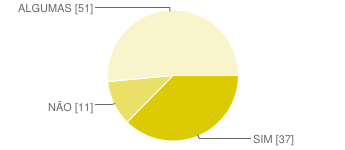
\includegraphics[scale=0.7]{imagens/fig4.png} 
\caption{As disciplinas de matemática atendem as necessidades das disciplinas de computação?}
\end{figure}

As necessidades dos 51\% dos alunos pode não serem atendidas por falta do bom aproveitamento das disciplinas, onde apenas 28\% deles consideram seu aprendizado ótimo ou bom, veja Figura 6, nessa imagem percebe-se a grande dificuldade dos alunos para assimilarem os conceitos matemáticos, essa deficiência pode acarretar no mau aproveitamento de algumas disciplinas específicas da computação (que exigirem uma base matemática), como por exemplo Computação Gráfica, Processamento de Imagens e Projeto e Análise de Algoritmos. Esse problema pode ser agravado pela falta de contextualização dos conceitos matemáticos, onde se continuarmos considerando um grau bom entre 8-10, ficaremos com apenas 22\% (Figura 5), esse deficit de 78\% pode ser um fator determinante do baixo desempenho dos alunos. 


\section{Trabalhos Relacionados}
\subsection{Algumas ferramentas de software voltadas para o ensino de Matemática} 
\begin{itemize}
\item GeoGebra - É um aplicativo de matemática dinâmica que combina conceitos de geometria e álgebra em uma única GUI. Sua distribuição é livre, nos termos da GNU General Public License, e é escrito em linguagem Java, o que lhe permite estar disponível em várias plataformas. O programa permite realizar construções geométricas com a utilização de pontos, retas, segmentos de reta, polígonos etc., assim como permite inserir funções e alterar todos esses objetos dinamicamente, após a construção estar finalizada. Equações e coordenadas também podem ser diretamente inseridas, é capaz de lidar com variáveis para números, pontos, vetores, derivar e integrar funções, e ainda oferecer comandos para se encontrar raízes e pontos extremos de uma função.

\item Cabri Geometry - É um software de construção que oferece “régua e compasso eletrônicos”, sendo a interface de menus de construção em linguagem clássica da Geometria. Os desenhos de objetos geométricos são feitos a partir das propriedades que os definem Apresenta interface dinâmica e interativa (‘desenhos em movimento’ e que podem ser automatizados através do recurso de ‘botões’); múltiplas representações (trabalha com geométrica sintética e um pouco de analítica); capturação de procedimentos (tem comando que permite ter acesso a história da construção e comandos para criação de macros).

\item GrafEq - um software que trabalha com equações e inequações, em coordenadas cartesianas e polares, possibilitando o desenho de curvas e regiões no plano cartesiano. Esses gráficos são gerados tomando como base a “Aritmética de Tupper”, com isso detectando pontos isolados em gráficos descontínuos automaticamente, sendo isso seu grande diferencial.

\item MatLab – voltado para o cálculo numérico, integrando análise numérica, cálculo com matrizes, processamento de sinais e construção de gráficos, seu diferencial é que a solução dos problemas são expressas somente como eles são escritos matematicamente. É programado na linguagem MATLAB, ou como é conhecido M-code. Bastante utilizado no ensino da álgebra linear e análise numérica.

\item R-Project - é uma linguagem e um ambiente de desenvolvimento integrado, para cálculos estatísticos e gráficos. É largamente usada entre estatísticos e data miners para desenvolver software de estatística e análise de dados. inquéritos e levantamentos de data miners, não sendo muito utilizado em ensino aprendizagem do uso da estatística.

\item Mapĺe - é uma linguagem de computação algébrica e simbólica. Como é frequente nos sistemas de álgebra computacional, as expressões simbólicas são armazenadas na memória como grafos acíclicos dirigidos. É comercializado como uma ferramenta de produtividade essencial para profissionais técnicos. Não sendo muito utilizado no processo de ensino -aprendizagem, mesmo assim muitos professores universitários o indicam para melhor entendimento nas resoluções de questões.
\end{itemize}

\subsection{Comparação entre TIC’s voltadas para o ensino-aprendizagem da matemática}
 
Devido a grande dificuldade encontrada nos alunos do curso de computação da Universidade Federal de Alagoas em todos os seus níveis, sendo isso um dos principais motivos de abandono do curso, decidimos investigar como poderíamos auxiliar nesse processo de aprendizagem.

Focamos em procurar meios que possam auxiliar a professores e principalmente alunos no processo de ensino-aprendizagem dessas matérias e um dos meios encontrados, foi o uso da própria tecnologia estudada por eles. Pesquisamos sobre ferramentas computacionais que impulsionem essa aprendizagem.

Encontramos em nossa pesquisa um número grande de ferramentas com este objetivo, para os variados nives de aprendizagem, seja esta no nível fundamental, médio ou superior.   Devido a  extensa quantidade de aplicações disponíveis, separamos inicialmente em dois grupos: Os que  obtivemos sucesso nos testes, ou seja, conseguimos download e  instalação, e os que não obtivemos sucesso.
Das ferramentas testadas, os insucessos foram:
        \begin{itemize}

            \item MatLab: por ser software proprietário, o download da aplicação depende do usuário estar logado e ter pago por seu uso.  Conseguimos entrar no site e verificar suas funcionalidades, entretanto não conseguimos efetuar o download da aplicação para efetuarmos os testes. $http://www.mathworks.com/products/matlab$
 
            \item Maple - Foi conseguido efetuar o download, porém na hora da instalação, foi pedido uma extensão Java que não foi encontrada. Foi visitado o site e verificado suas funções e formas de uso. É um programa profissional, entretanto foi encontrado no site uma nota informando que futuramente será disponibilizado uma versão acadêmica. $http://www.maplesoft.com/support/downloads/m17_02update.aspx$
            
            \item Derive - Conseguimos entrar no site que explica suas principais funcionalidades, entretanto o link do download estava quebrado e não conseguimos instalar para realizarmos os testes. $http://derive.br.uptodown.com$
            
            \item Curve Expert - Suas principais aplicações foram conseguidas no site, porém não conseguimos efetuar o download para realizarmos os testes. $http://www.curveexpert.net/download$
            
            \item Nulcalc - Não foi possível testar esta aplicação porque ocorreram erros durante sua instalação. O programa não se mostrou compatível com o Windows7 e nem com o Ubuntu14. $http://www.dartmouth.edu/comp/soft-comp/software/downloads/windows/nucalc-wp.html$
            
            \item LogPaper - Não foi possível testar esta aplicação porque ocorreram erros durante sua instalação. O programa não se mostrou compatível com o Windows7 e nem com o Ubuntu14. $http://log-paper.softonic.com.br$
            
            \item Kpercentage - Esta aplicação está disponível somente para distribuições Linux. Obtivemos sucesso no download, mas durante a instação ocorreu o erro “dependency is not satisfiable”. $http://wiki.ubuntu-br.org/KPercentage$
        \end{itemize}
        
Das ferramentas que foram testadas, isto é, que tiveram download e instalação com sucesso, dividimos em grupos por área de assunto. As ferramentas que trabalham mais de um assunto, aparecerá em mais de um grupo.
         \begin{itemize}
            \item Geometria Plana
            \begin{itemize}
                \item Geogebra - por tratar-se de ser um software de geometria dinâmica, GeoGebra uma das ferramentas que permite ao usuário perceber graficamente as mudanças que ocorrem ao alterar as coordenadas de um ponto. Essa ferramenta tanto trabalha com geometria no plano cartesiano (2D) como no espaço (3D), os métodos de entrada podem ser: equações, interseção de pontos ou retas para a construção de figuras:
                
\begin{quotation}
Um exemplo simples apresentado em sala, que pode ilustrar o “dinamismo” desta geometria é a construção de um triangulo retângulo. Para construir basta colocar os ter pontos no plano cartesiano. Constrói o triangulo ABC, sendo e o torna polígono, onde o próprio Geogebra colocará todos as medidas e nomes automaticamente, no nosso caso os pontos são A(1,5), B(1,1) e C(5,1) (figura 1:exemplo 1.1). Uma vez efetuada a construção podemos mover os pontos A ou B ou C pela área de desenho e o programa que implementa a GDI, automaticamente, redesenhará todos os objetos preservando suas propriedades.\end{quotation}\citep{cardoso2010software}

\begin{figure}[!h]
\centering
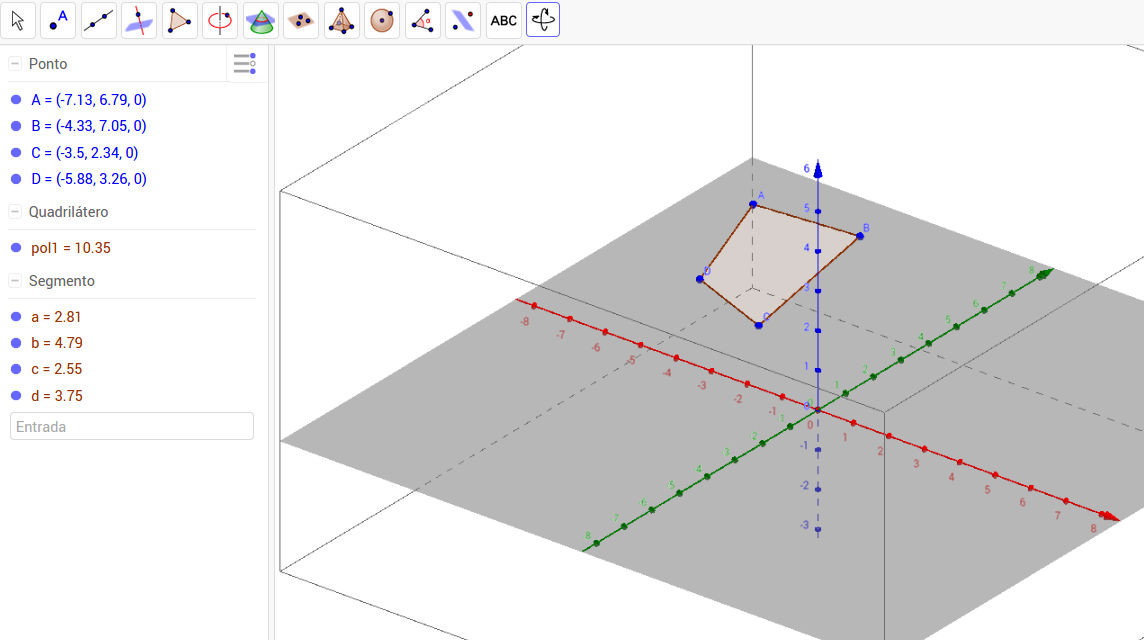
\includegraphics[scale=0.23]{imagens/geo.jpg} 
\caption{Imagem da versão online do GeoGebra}
\end{figure}

\item GeoNext - Esta ferramenta permite a criação e manipulação de figuras geométricas através de inserção de pontos, linhas, círculos, setas, por meio de seleção na área de desenho ou por escrita de equações.
\begin{quote}
"Principalmente voltado para os conceitos geométricos, o software Geonext permite a construção de figuras geométricas de maneira interativa". (CARDOSO, 2010).
\end{quote}

\begin{figure}[!h]
\centering
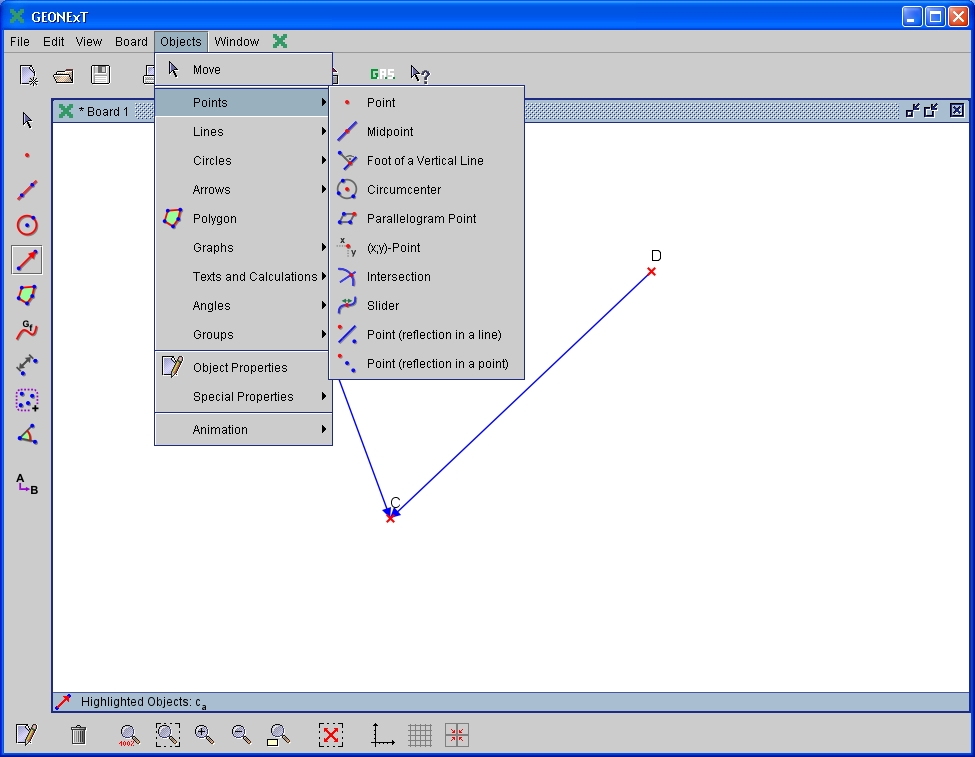
\includegraphics[scale=0.23]{imagens/geonext.png} 
\caption{Imagem do GeoNext}
\end{figure}

\item Modellus - O Modellus tem foco na criação e manipulação de modelagem computacional, sua especialidade está na construção de gráficos, entretanto esta aplicação permite aos usuários criarem figuras geométricas como polígonos, retas e círculos no plano. Utiliza método de inserção através equações.
    Uma das principais funcionalidades é a criação de figuras geométricas dinâmicas, ou seja, animações que mostram as mudanças que ocorrem na imagem quando é alterada a posição de um ponto no plano.

\item WinPlot - O WinPlot só permite a plotagem de figuras geométricas em 2D e 3D, vetores e funções através de inserção de equações, ou seja, não é permitido que o usuário clique na janela para criar um ponto. As equações que são digitadas na entrada de dados são predefinidas, assim, a aplicação evita erros cometidos pelos usuário, ou seja, mostra ao usuário a estrutura permitida.

\item Kaleido Tile - Indicado para o ensino de geometria (plana euclidiana e hiperbólica). Ele possui formas predefinidas, ou seja, não é possível entrada de dados por inserção de equações. Portanto ele tem um número muito pequeno de figuras disponíveis para estudo. É um software simples, voltado para crianças.

\begin{figure}[!h]
\centering
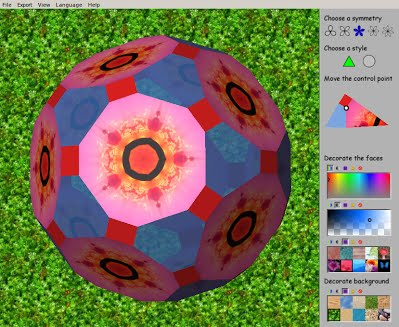
\includegraphics[scale=0.6]{imagens/tile.jpg} 
\caption{Imagem do Kaleido Tile}
\end{figure}

\item s3D SecBuilder - Possui um conjunto finito de figuras geométricas, contudo, não é possível inserir outras formas, ou seja, só é permitido o uso de formas geométricas predefinidas. Como Kaleido Tile, o  s3D SecBuilder tem como usuário alunos dos primeiros anos do ensino fundamental. 

\begin{figure}[!h]
\centering
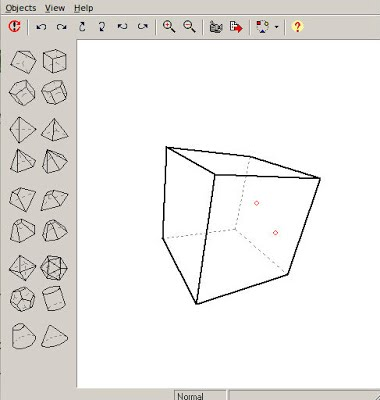
\includegraphics[scale=0.45]{imagens/s3.jpg} 
\caption{Imagem do s3D SecBuildere}
\end{figure}

\item Zomecad - É uma ferramenta totalmente dedicada a criação de formas geométricas em 3D. Zomecad possui  entada de dados através de seleção de pontos e retas para formar as imagens.

\begin{figure}[!h]
\centering
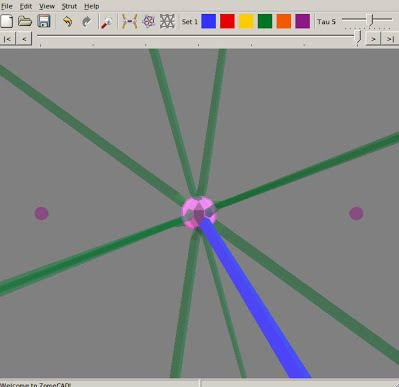
\includegraphics[scale=0.45]{imagens/zz.jpg} 
\caption{Imagem do Zomecad}
\end{figure}

\item Kig - Possui ótimas funcionalidades na área da geometria em 2D. Pode ser utilizado tanto no ensino fundamental, médio e superior. É possível exportar as imagens geras no programa em dois formatos:  LaTeX e SVG (linguagem XML).

\item Cabri Geometry - Diferente dos demais softwares neste tópico de aplicações que criam formas geométrias, este é um dos mais simples. Possui poucas opções de figuras geométricas predefinidas quando comparado as demais aplicações desta seção. Entretanto ele cumpre (mesmo que de maneira simples) os requisitos básicos para uso em sala de aula ou para criação de formas geométricas básicas.

\item Cinderella - É uma aplicação que contém diversas possibilidades de manipulação e criação de formas geométricas em 2D. A entrada de dados é através de seleção de formas geométricas predefinidas e/ou seleção de pontos, retas. A aplicação permite aos usuários exportarem seus gráficos e imagens geradas no programa nos seguintes formatos: pdf, jpeg, html e png.

\begin{figure}[!h]
\centering
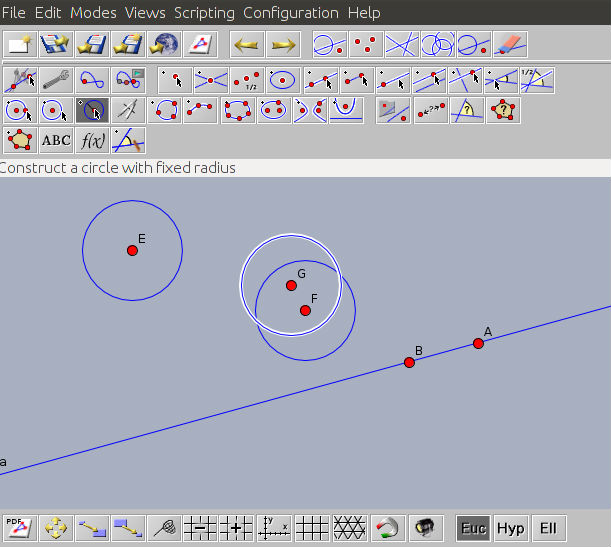
\includegraphics[scale=0.35]{imagens/cinderella.jpg} 
\caption{Imagem do Cinderella}
\end{figure}

\item Sketchpad - Este software apesar de ser pago, possui versão para de testes disponível para estudantes e professores. Sua principal funcionalidade é a criação de formas geométricas. A entrada de dados dar-se através de seleção de formas predefinidas e pontos que ligados formam uma ou mais formas.

\begin{figure}[!h]
\centering
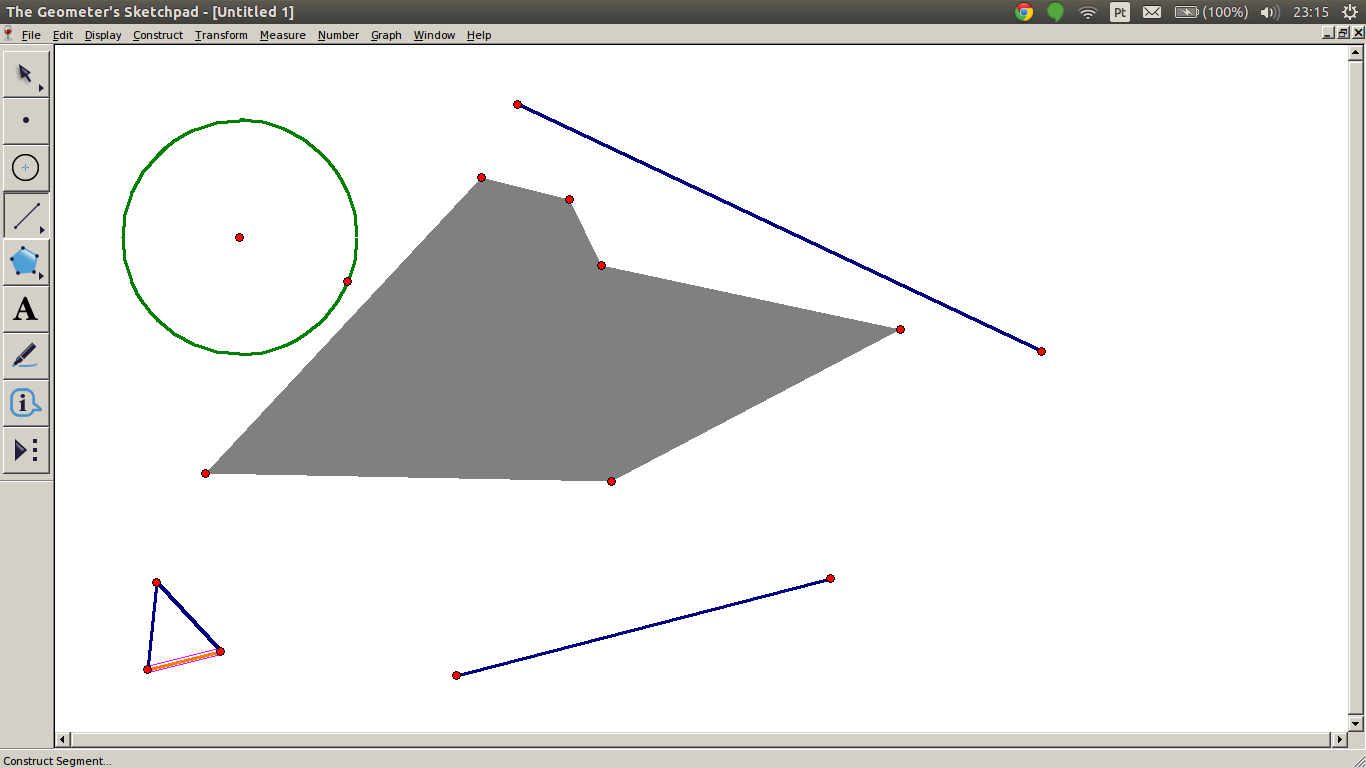
\includegraphics[scale=0.15]{imagens/Sketchpad.png} 
\caption{Imagem do Sketchpad}
\end{figure}

\end{itemize}

\item Funções, Limites e Derivadas

Para a disciplina onde é visto o estudo de limites e derivadas, foram encontradas as seguintes ferramentas para auxiliarem aos alunos ao melhor entendimento:
\begin{itemize}
\item  Geogebra – Utiliza a linguagem do LaTeX, porém mostra de forma bem clara o processo de derivação de uma função, o gráfico é bem demonstrado na tela facilitando o entendimento do que seria a derivação e da importância do limite para tal.


\item Xfunctions - É uma aplicação que permite explorar funções e as respectivas propriedades. O utilizador pode definir uma função e visualizar a sua representação gráfica, a expressão e ainda a tabela de valores. Entre outras opções, possibilita o estudo das derivadas de funções. Existe somente a versão para Mac.

\item VisualMethods - É uma aplicação que possibilita a representação gráfica de funções de uma variável, calcula o valor numérico de integrais, mostra a área, integra equações diferenciais e faz interpolação. É muito eficaz na iniciação do estudo de integralização.

\item Mathematica - Envolve muitos temas da matemática, inclusive a parte de simplificação polinomial e limites, facilitando ao aluno a entender melhor o processo de limitação de uma função. A nova versão do programa, versão 10, possibilita ao usuário a trabalhar na nuvem.

\item GraphMat - Este programa possibilita a representação gráfica de funções (incluindo as polares, paramétricas, logaritmicas, desigualdades, etc). Possibilita ainda que encontre a derivada e a respectiva representação gráfica da função definida, o integral, etc.

\item Advanced Grapher - Permite a representação gráfica de variadas funções, incluindo as funções implícitas, desigualdades, etc. Possibilita ainda a apresentação dos valores de uma função em tabelas, determinar a derivada, tangente, etc.
\end{itemize}
\item Álgebra Linear

Os programas relacionados a seguir, isto é, aqueles relacionados na lista, (testado ou não) é de uso paralelo a aprendizagem da matéria de Álgebra Linear.

\begin{itemize}
\item MatLab - É a linguagem de alto nível e um ambiente interativo usado por milhões de engenheiros e cientistas de todo o mundo. Ele permite que você explore e visualize ideias e colabora em todas as disciplinas, incluindo processamento de imagem, comunicações, sistemas de controle e finanças computacionais, e tem uma grande utilidade em Álgebra Linear.

\item Maple - O Maple é um sistema de álgebra computacional comercial de uso diversificado. É um aplicativo bem completo, tendo em vista que trabalha com "pacotes", tais como student, plots, linalg, geometry, entre outros. Cada pacote é um conjunto de comandos que o Maple possui para trabalhar dentro de um assunto específico, como por exemplo, para plotar gráfico, deve-se fazer a chamada do pacote plots escrevendo a linha de comando with(plot).

\item Derive -  É uma aplicação destinada a qualquer estudante, professor ou profissional que tem de fazer qualquer tipo de tarefa relacionada com matemática. Pode fazer complexos exercícios de matemática e álgebra, rápida e apuradamente. Funciona com matrizes e vectores numa interface muito fácil e confortável. Também representa qualquer tipo de gráfico ou esquema.

\end{itemize}
\end{itemize}

\section{Escolhas tecnológicas}

\subsection {Controle de versão}
A escolha de um controles de versão que será utilizado no projeto, deu-se através de estudo sobre as ferramentas mais utilizadas atualmente, algumas delas foram:
\begin{itemize}
\item GIT
\item Mercurial
\item Subversion
\item VSC
\item ClearCase
\end{itemize}
Optamos pela ferramenta git, pois:

\begin{enumerate}
\item Pode ser utilizada com github, que é uma “rede social” para programadores.
\item Possui a escolha de um repositório público.
\item Variedade de escolha da licença do projeto (A licença do projeto é GPLv3).
\end{enumerate}

\subsection {Licença de Uso}

Neste tópico será apresentado algumas licença de uso de software.

\begin{itemize}
\item Open Source:
\begin{itemize}
\item Distribuição livre.
\item Acesso ao código-fonte.
\item Permissão para criação de trabalhos derivados.
\item Integridade do autor do código-fonte.
\item Não discriminação contra pessoas ou grupos.
\end{itemize}

\item BSD (Berkeley Software Distribution):
\begin{itemize}
\item Licença de código aberto.
\item Possui menos restrições que a GPL.
\item Tem domínio público.
\item Pode ser incorporado a produtos proprietários.
\end{itemize}


\item GPL ( Licença Pública Geral):
\begin{itemize}
\item A liberdade de executar o programa, para qualquer propósito.
\item A liberdade de estudar como o programa funciona e adaptá-lo para as suas necessidades.
\item A liberdade de redistribuir cópias de modo que você possa ajudar ao seu próximo.
\item A liberdade de aperfeiçoar o programa, e liberar os seus aperfeiçoamentos, de modo que toda a comunidade se beneficie deles.
\end{itemize}

\item GPLv1:
\begin{itemize}
\item Viola a licença quem distribui o programa impondo restrições adicionais a quem o receba direta ou indiretamente.
\item Negar acesso ao código fonte.
\end{itemize}

\item GPLv2:
\begin{itemize}
\item Qualquer obrigação de restringir a liberdade de outros implica não poder distribuir o programa.
\item Proibido distribuir programa recebido, desacompanhado dos fontes.
\item Quem recebe software livre em protocolos P2P, como bittorrent, pode estar violando a GPLv2.
\end{itemize}

\item GPLv3:
\begin{itemize}
\item Permite distribuição sem fontes, sem exigir aceitação dos termos da licença (é proibido na GPLv2), desde que a informação sobre como obter os fontes correspondentes seja disponibilizada.
\item Pela facilidade, pois tem diversos software que possibilita o uso do github através de interface gráfica (GUIS clients).
\item Possui plugin que pode ser utilizada em conjunto com algumas IDE's.
\end{itemize}
\end{itemize}

\subsection{IDE}

A escolha da IDE que será utilizado no projeto é a ferramenta Eclipse. Vários fatores ajudaram nesta decisão, entre elas estão:
\begin{itemize}
\item Facilidade de uso
\item Eclipse possui um plugin (Egit) para conexão com o github.
\item Suporte a várias linguagens de programação.
\item Por ter licença GPL
\end{itemize}

\section{Resultado das entrevistas}

\begin{figure}[!h]
%\centering
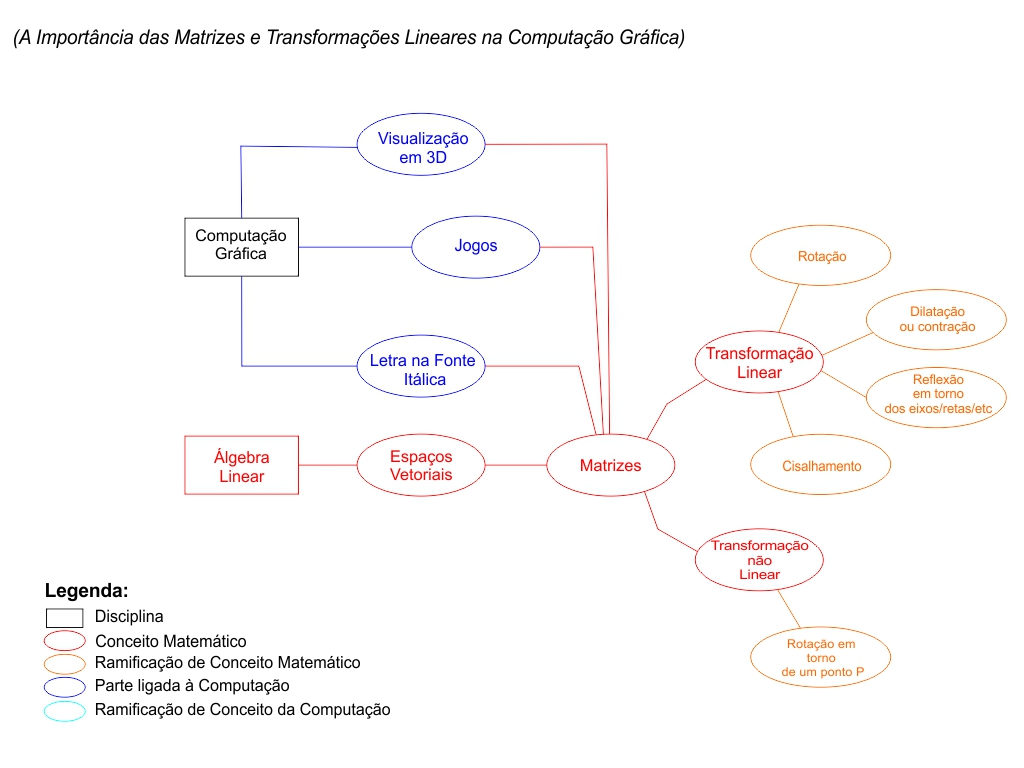
\includegraphics[scale=0.4]{imagens/DiagramaEXTRA.jpg} 
\caption{Diagrama que mostra a importancia do conhecimento de Matrizes e Transformações Lineares na Computação Gráfica}
\end{figure}

\begin{figure}[!h]
\centering
%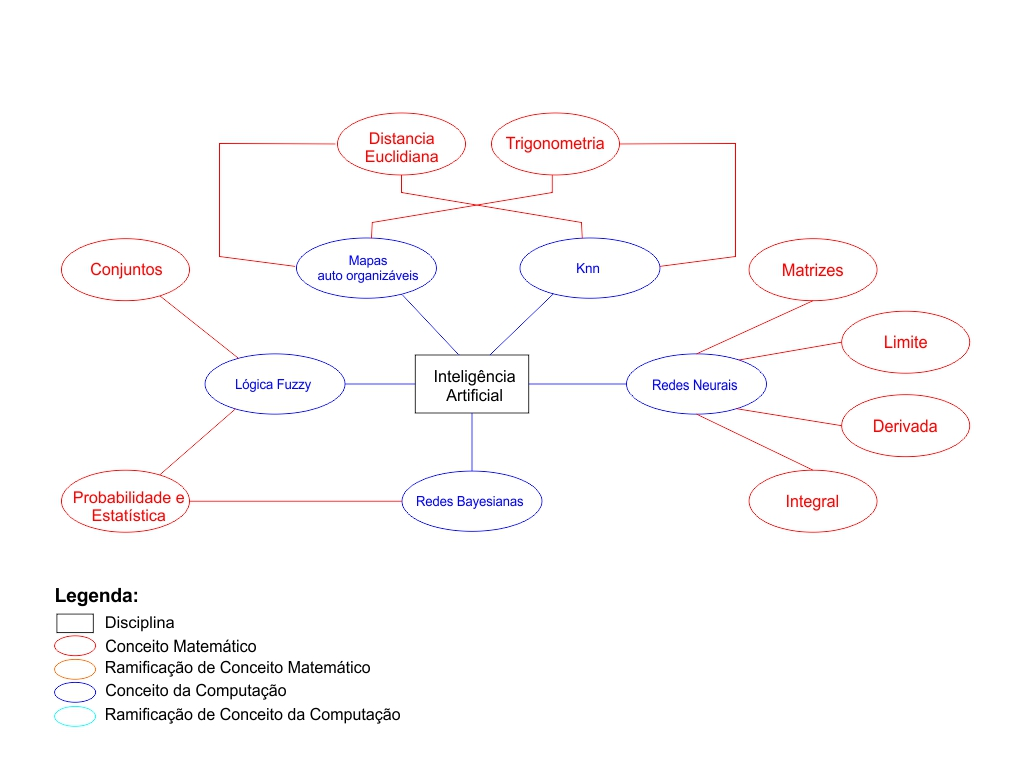
\includegraphics[scale=0.4]{imagens/Diagrama Inteligencia Artificial.jpg}
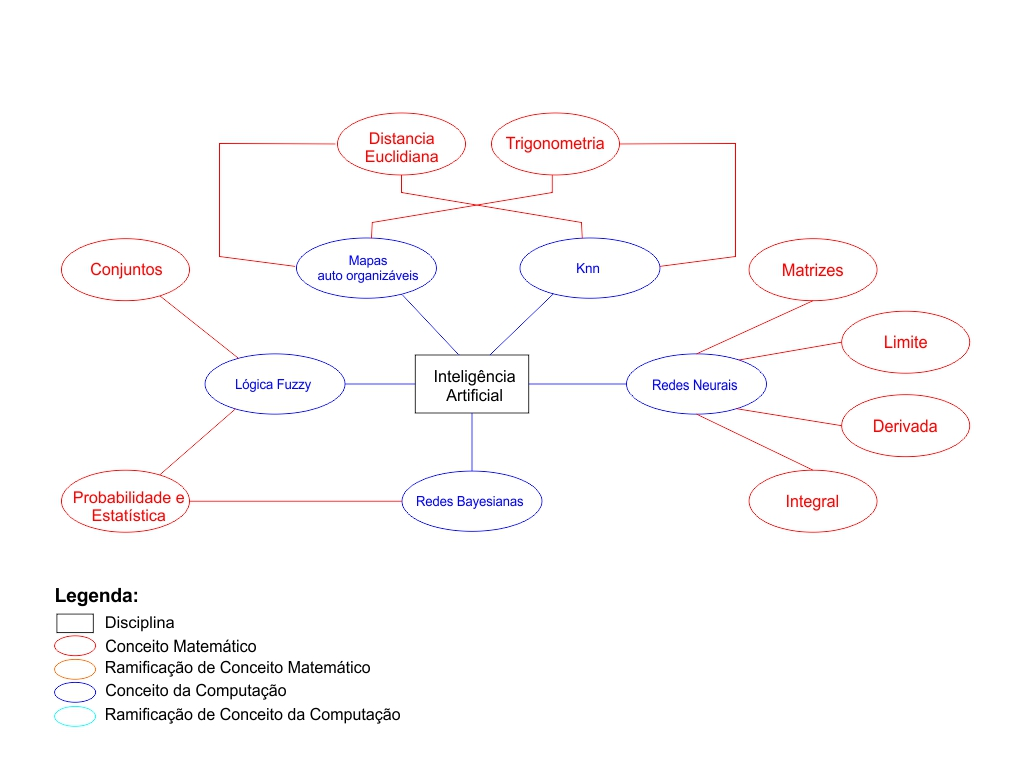
\includegraphics[scale=0.4]{imagens/IA.jpg} 
\caption{Diagrama da Disciplina de Inteligencia Artificial}
\end{figure}

\begin{figure}[!h]
	\centering
	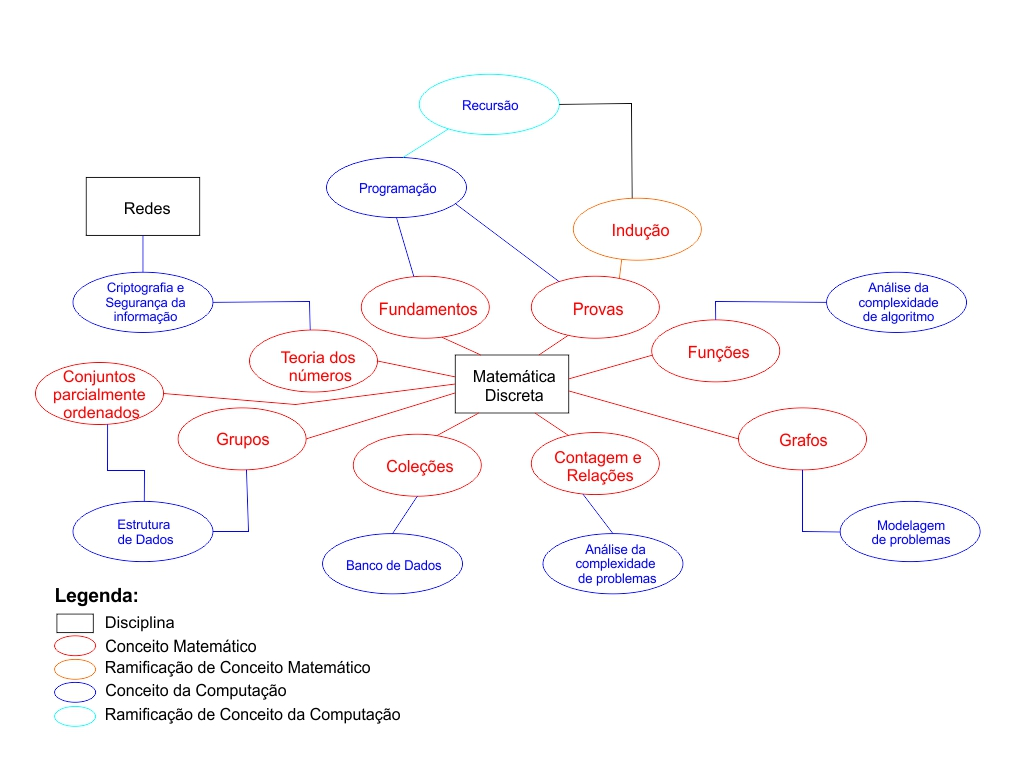
\includegraphics[scale=0.4]{imagens/MD.jpg} 
	\caption{Diagrama da Disciplina de Matemática Discreta}
\end{figure}

\begin{figure}[!h]
	\centering
	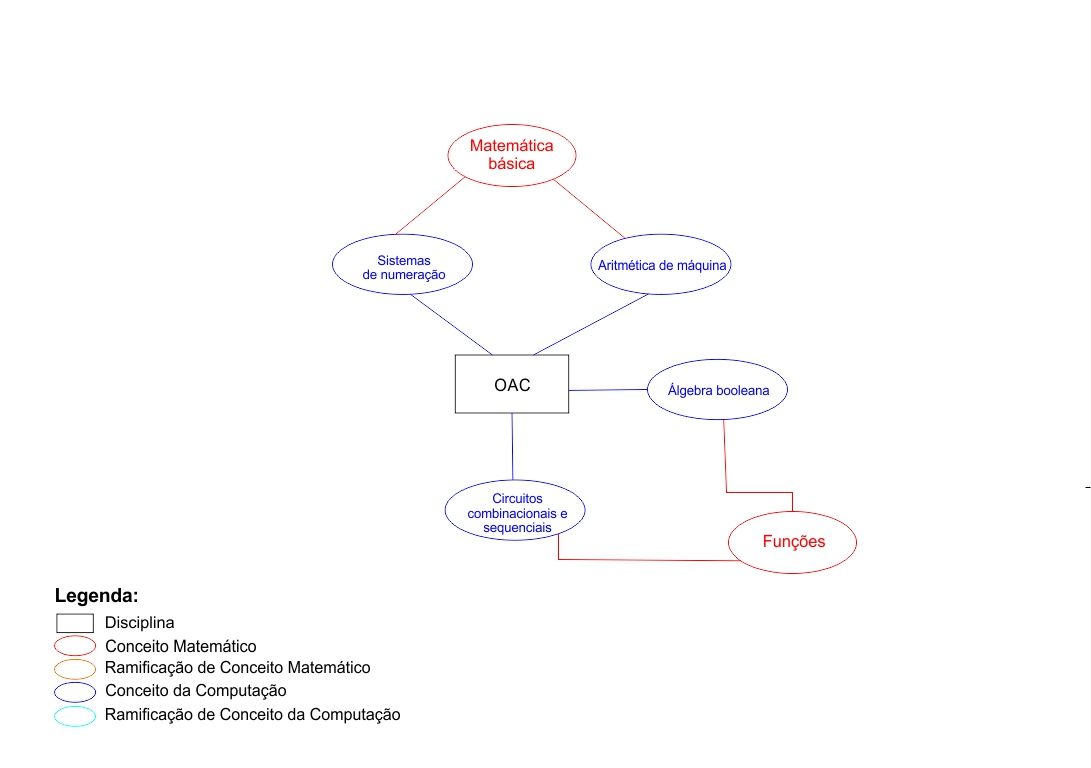
\includegraphics[scale=0.4]{imagens/OAC.jpg} 
	\caption{Diagrama da Disciplina de Organização e Arquitetura de Computadores}
\end{figure}

\begin{figure}[!h]
	\centering
	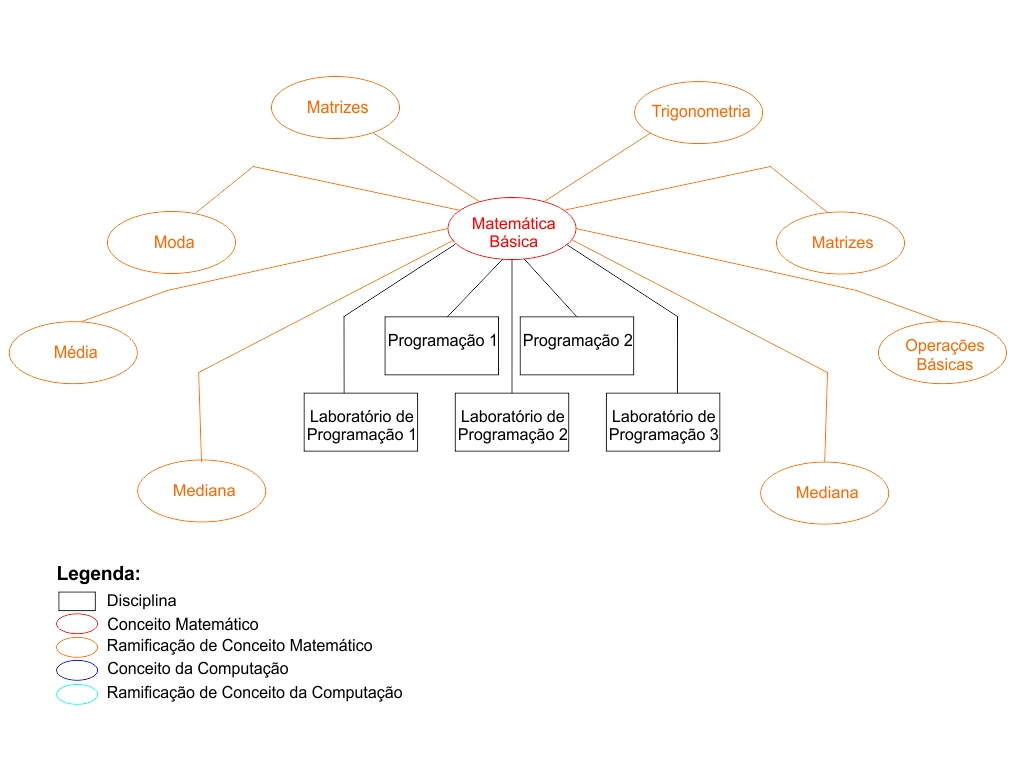
\includegraphics[scale=0.4]{imagens/Programacao.jpg} 
	\caption{Diagrama da Disciplina de Programação}
\end{figure}

\begin{figure}[!h]
	\centering
	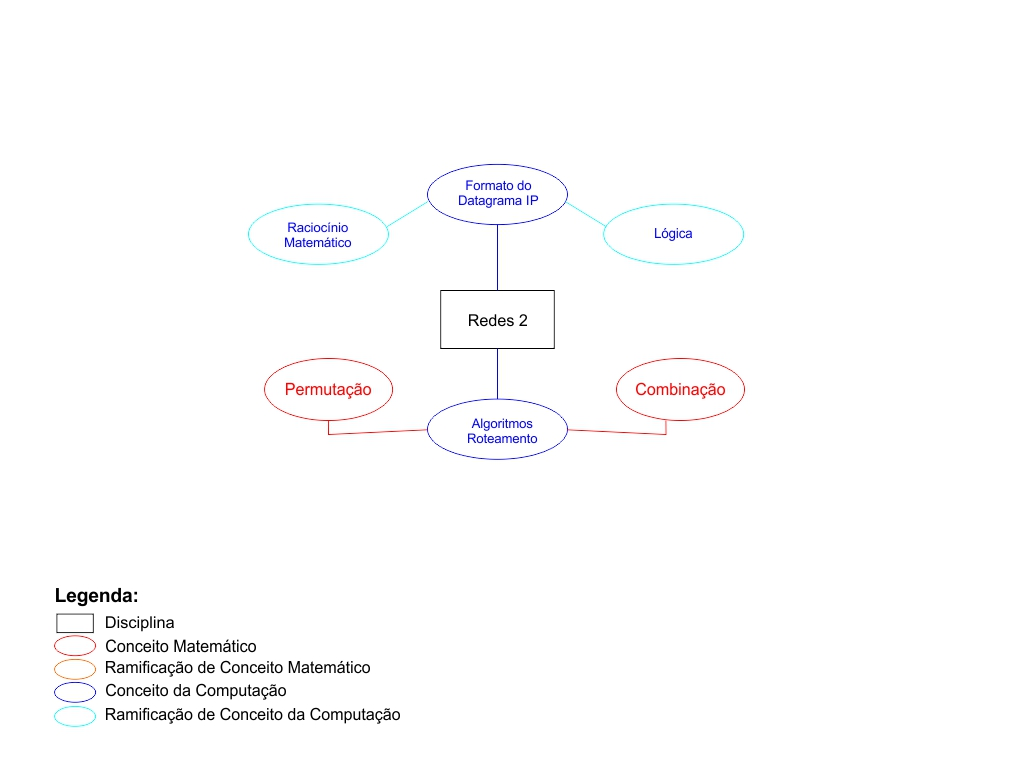
\includegraphics[scale=0.5]{imagens/R2.jpg} 
	\caption{Diagrama da Disciplina de Redes de Computadores II}
\end{figure}

\begin{figure}[!h]
	\centering
	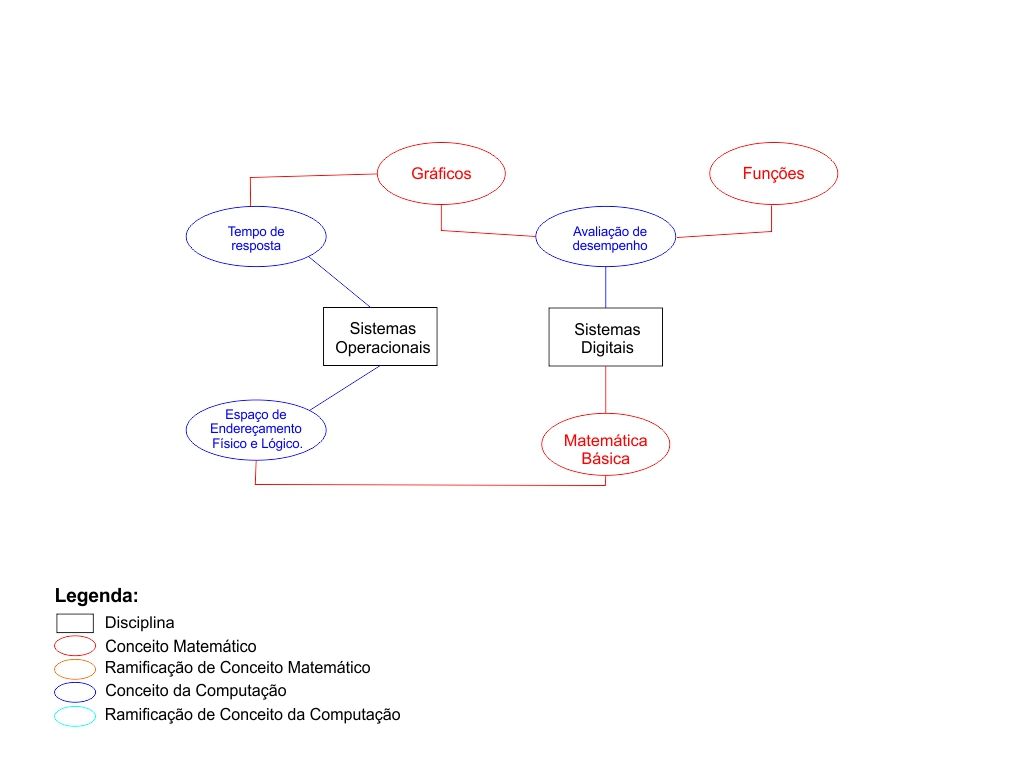
\includegraphics[scale=0.5]{imagens/SD.jpg} 
	\caption{Diagrama das Disciplinas de Sistemas Digitais e Sistemas Operacionais}
\end{figure}

\begin{figure}[!h]
	\centering
	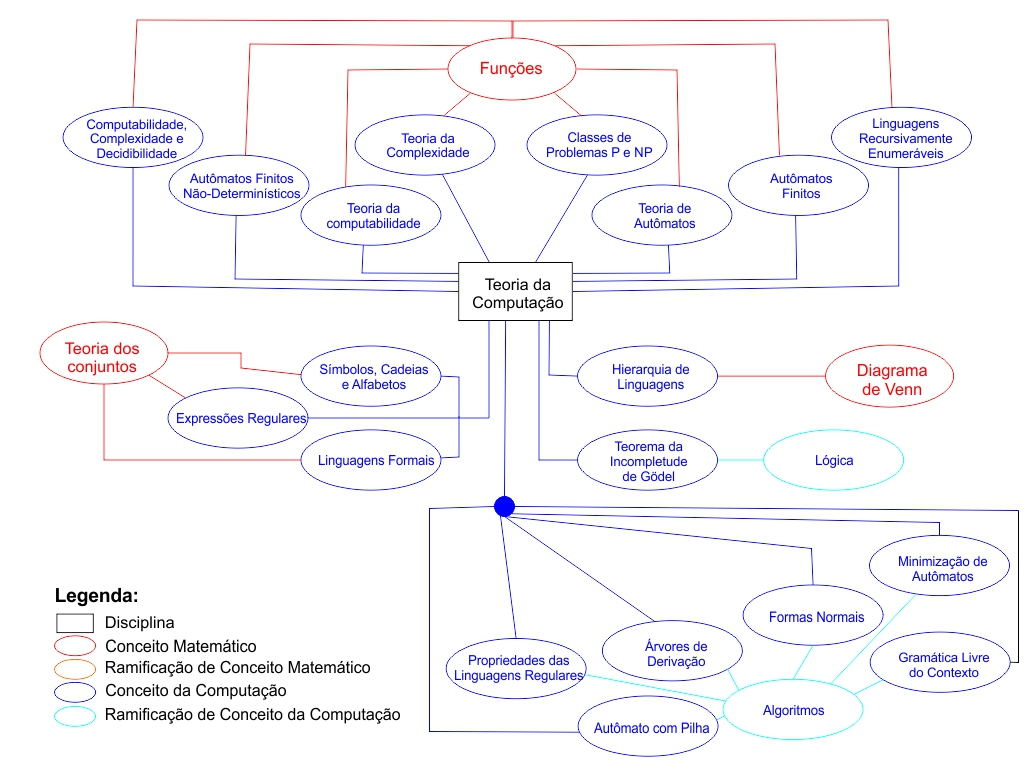
\includegraphics[scale=0.5]{imagens/TC.jpg} 
	\caption{Diagrama da Disciplina de Teoria da Computação}
\end{figure}

\begin{figure}[!h]
	\centering
	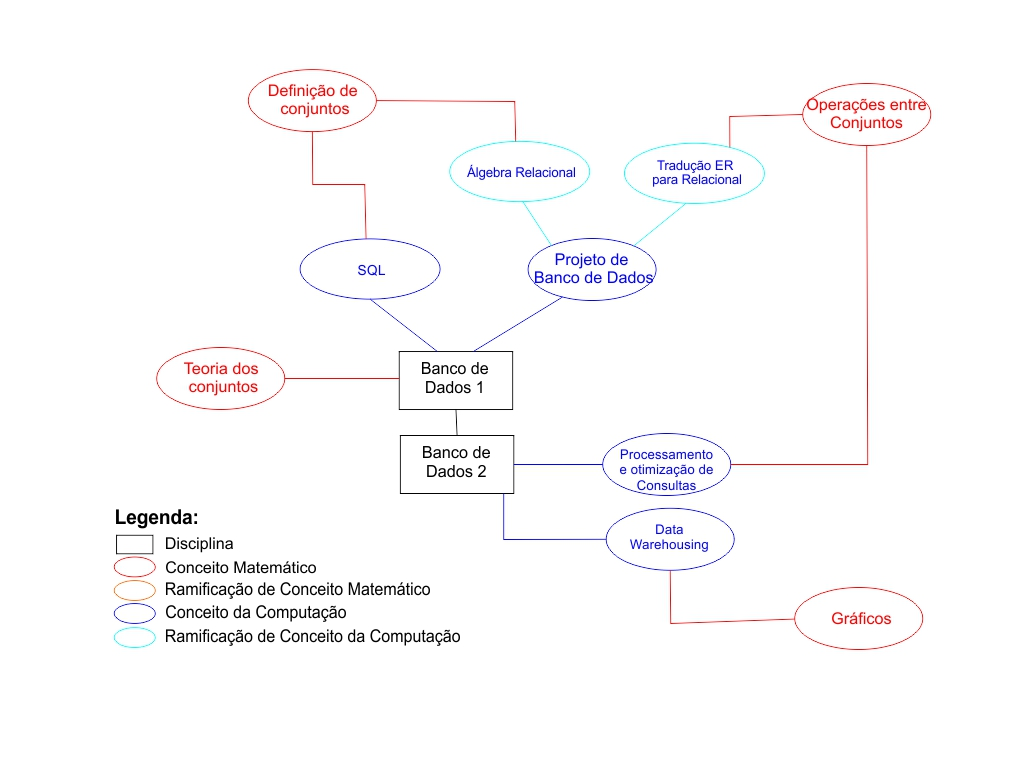
\includegraphics[scale=0.5]{imagens/BD2.jpg} 
	\caption{Diagrama das Disciplinas de Banco de Dados I e II}
\end{figure}

\begin{figure}[!h]
	\centering
	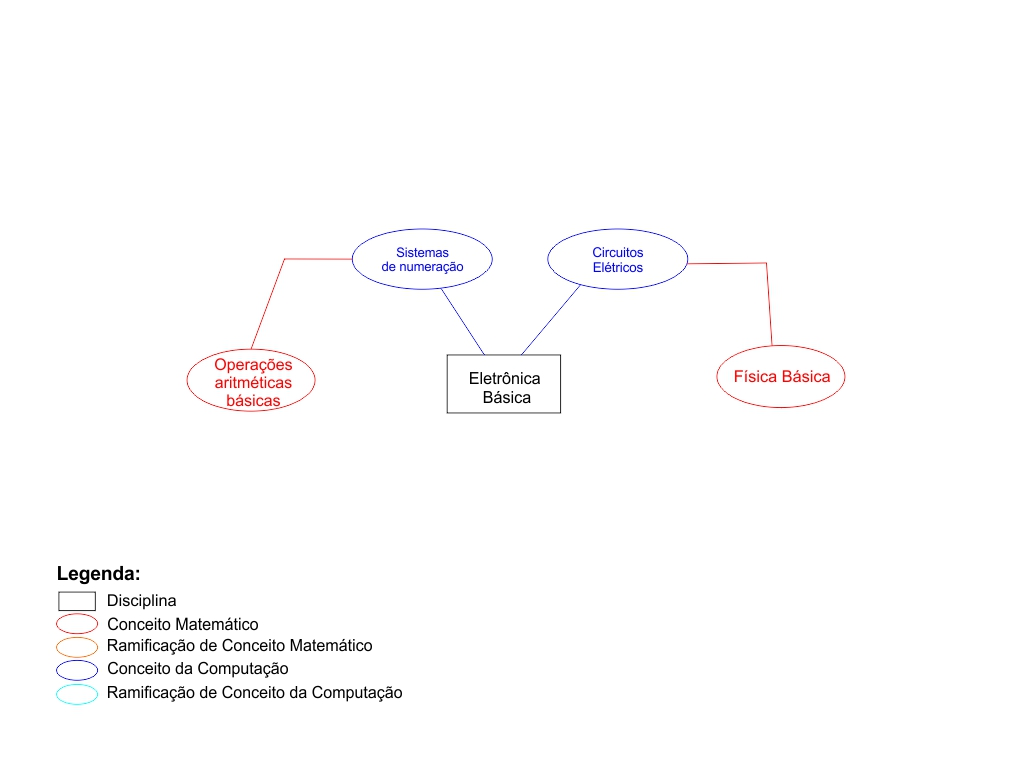
\includegraphics[scale=0.5]{imagens/EB.jpg} 
	\caption{Diagrama da Disciplina de Eletrônica Básica}
\end{figure}

\begin{figure}[!h]
	\centering
	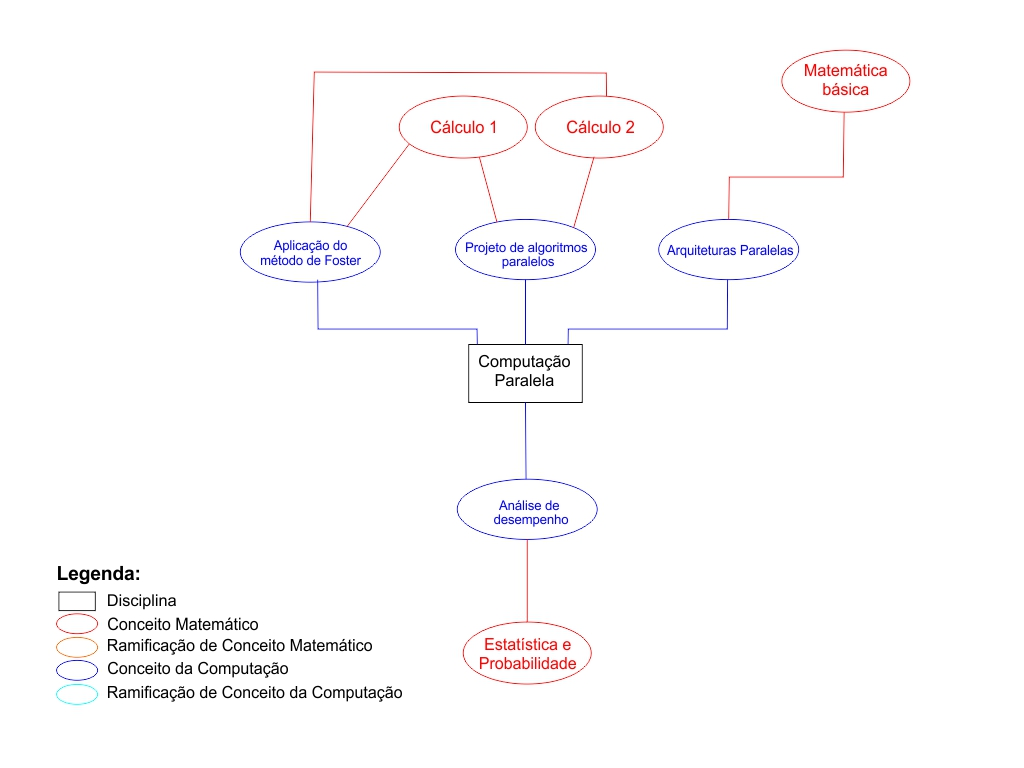
\includegraphics[scale=0.5]{imagens/CP.jpg} 
	\caption{Diagrama da Disciplina de Computacao Paralela}
\end{figure}

\begin{thebibliography}{9}
\bibliographystyle{plainnat}
\bibliography{references.bib}

\end{thebibliography}

\end{document}
